\chapter{Dados Detalhados da Avaliação Experimental}
\label{cap:dados-experimentais}

Este apêndice apresenta os dados completos coletados durante a avaliação
experimental do \textit{bot} educacional, incluindo gráficos gerados
automaticamente pelo Google Forms e tabelas com as respostas detalhadas dos
participantes.

\section{Questionário de Avaliação}
\label{sec:questionario}

O questionário foi aplicado aos 10 participantes do experimento após sua
participação nas sessões simuladas de aula remota. As perguntas abordaram
aspectos de usabilidade, eficácia pedagógica e percepção geral da ferramenta,
utilizando principalmente escala Likert de 1 a 5 pontos.

\section{Gráficos Gerados pelo Google Forms}
\label{sec:graficos-forms}

As figuras a seguir apresentam os gráficos gerados automaticamente pelo Google
Forms, correspondentes às respostas coletadas até o encerramento da coleta em
03/07/2025. Estes gráficos oferecem uma visualização imediata da distribuição
das respostas para cada pergunta do questionário.

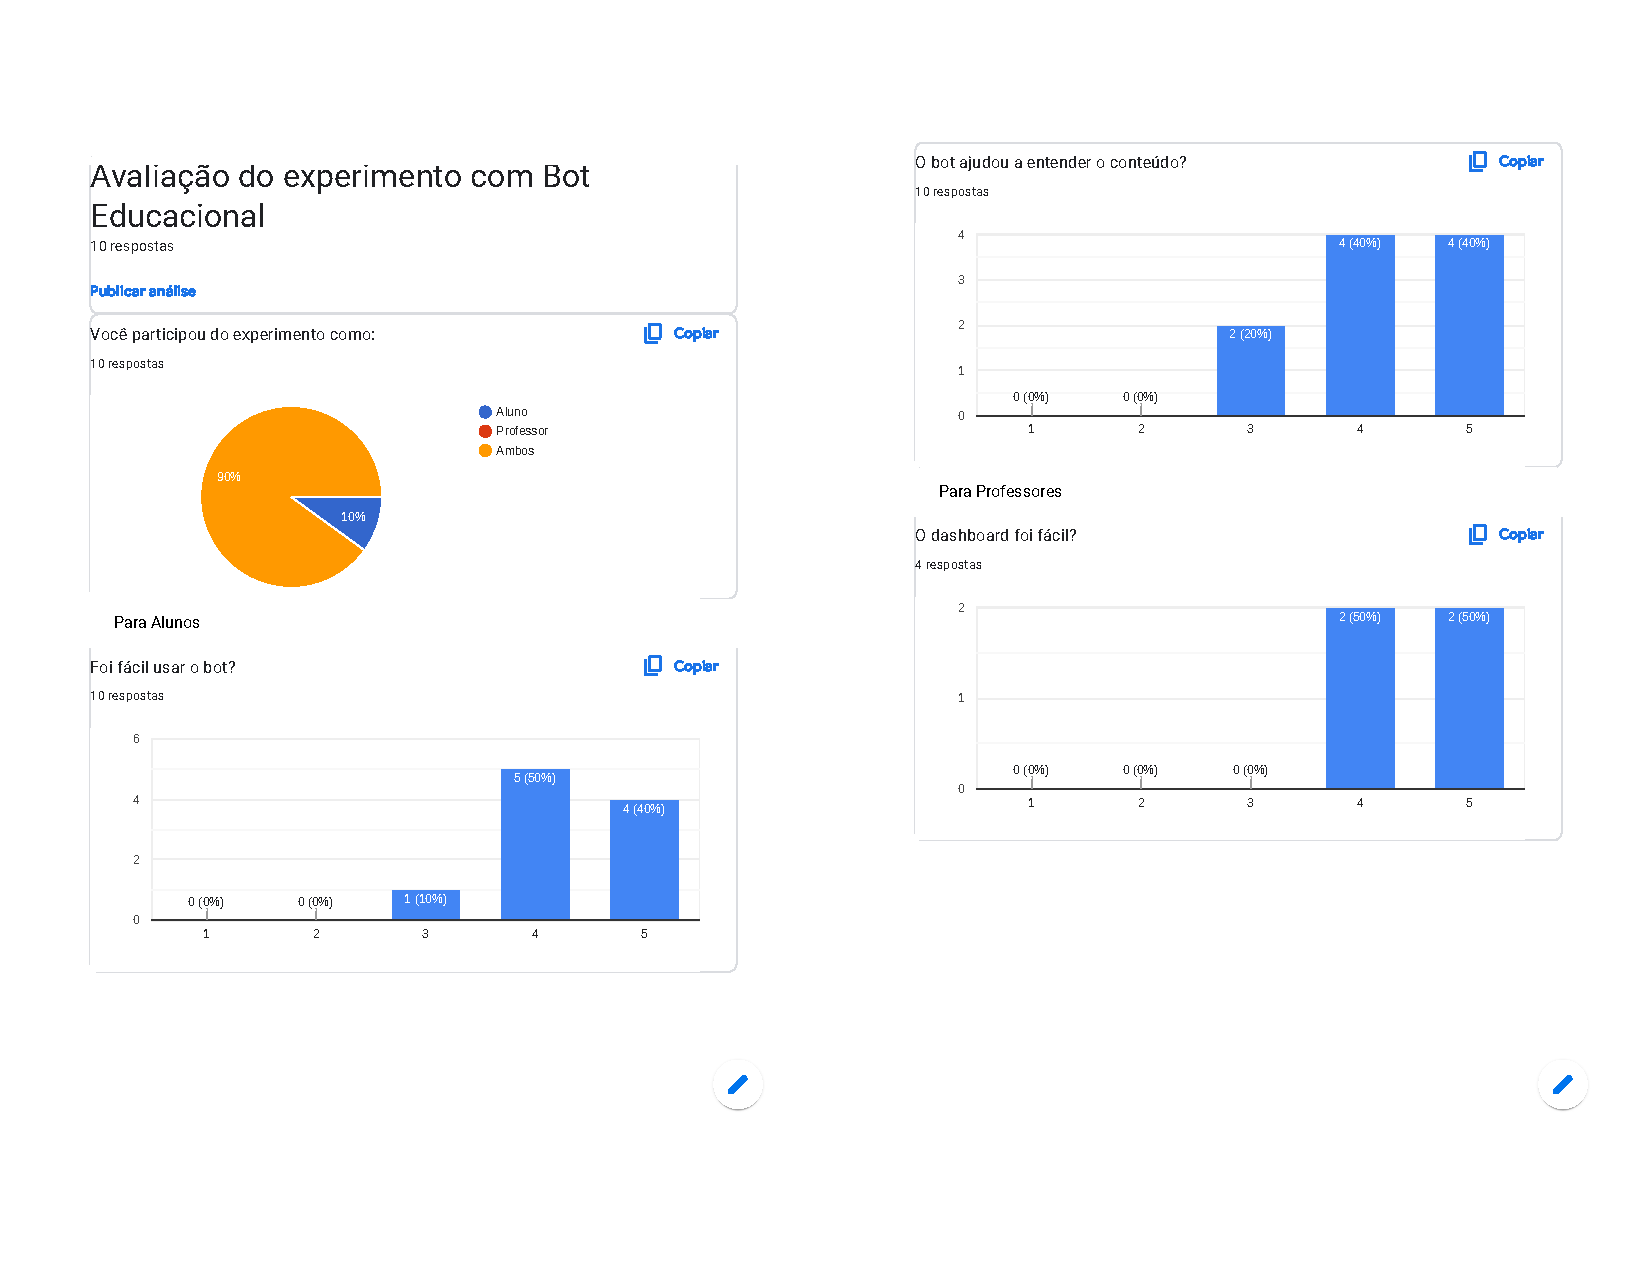
\includepdf[pages=-]{forms.pdf}

\section{Dados Tabulares Completos}
\label{sec:dados-tabulares}

Para facilitar análises futuras e garantir transparência na pesquisa, a Tabela
\ref{tab:respostas-completas} apresenta todas as respostas coletadas de forma
estruturada. Os dados incluem tanto as avaliações quantitativas quanto os
comentários qualitativos dos participantes.

\begin{table}[htb]
\centering
\caption{Síntese das respostas quantitativas coletadas}
\label{tab:respostas-completas}
\footnotesize
\begin{tabular}{|l|c|c|c|c|c|c|}
\hline
\textbf{Pergunta} & \textbf{Média} & \textbf{Min} & \textbf{Max} & \textbf{Notas 4-5} & \textbf{Total} \\
\hline
Facilidade de uso do bot & 4,3 & 3 & 5 & 80\% & 10 \\
\hline
Bot ajudou a compreender & 4,1 & 3 & 5 & 70\% & 10 \\
\hline
Dashboard foi fácil & 4,5 & 4 & 5 & 100\% & 6* \\
\hline
Dashboard ajudou monitorar & 4,2 & 3 & 5 & 83\% & 6* \\
\hline
Bot reduziu carga na aula & 3,8 & 3 & 5 & 60\% & 10 \\
\hline
Bot tornou aula interativa & 4,7 & 3 & 5 & 90\% & 10 \\
\hline
Facilitou comunicação & 4,7 & 4 & 5 & 100\% & 10 \\
\hline
Reduziu isolamento & 4,1 & 3 & 5 & 70\% & 10 \\
\hline
Usaria em mais aulas & 4,6 & 4 & 5 & 100\% & 10 \\
\hline
\end{tabular}
\begin{flushleft}
\footnotesize
*Apenas participantes que utilizaram o dashboard responderam estas perguntas.
\end{flushleft}
\end{table}

\section{Comentários Qualitativos}
\label{sec:comentarios-qualitativos}

Os comentários dos participantes foram categorizados em aspectos positivos e
sugestões de melhoria, conforme apresentado nas seções seguintes.

\subsection{Aspectos Mais Valorizados}
\label{subsec:aspectos-positivos}

Os participantes destacaram consistentemente os seguintes aspectos:

\begin{itemize}
\item \textbf{Anonimato}: "Poder comentar em anônimo e não ser necessário
responder em áudio" (Participante 2)
\item \textbf{Interatividade}: "Interatividade com o uso do dashboard"
(Participante 7)
\item \textbf{Facilidade de comunicação}: "Poder responder digitando e não
precisar falar" (Participante 3)
\item \textbf{Redução de constrangimento}: "Permite que você faça perguntas sem
que seus colegas julguem você" (Participante 6)
\end{itemize}

\subsection{Principais Sugestões de Melhoria}
\label{subsec:sugestoes-melhoria}

As sugestões mais recorrentes incluem:

\begin{itemize}
\item \textbf{Interface mais intuitiva}: "Uma maneira mais fácil de responder
coisas sem ter que usar comandos, por exemplo, botão" (Participante 4)
\item \textbf{Respostas inline}: "Perguntas e respostas poderiam ser inline
como '/ask minha pergunta 123?'" (Participante 6)
\item \textbf{Notificações}: "Aparecer notificações pro professor quando chega
pergunta" (Participante 10)
\item \textbf{Controle de moderação}: "Opção de bloquear perguntas anonimizadas,
já que tem gente que pode se aproveitar" (Participante 6)
\end{itemize}

\section{Considerações Metodológicas}
\label{sec:consideracoes-metodologicas}

É importante notar que este experimento foi conduzido em ambiente controlado
com duração limitada. Os dados apresentados refletem impressões iniciais dos
participantes e podem não capturar completamente os efeitos de uso prolongado
da ferramenta em contextos educacionais reais.

Os resultados devem ser interpretados considerando as limitações inerentes ao
método experimental utilizado, conforme discutido na Seção
\ref{sec:limitacoes-conclusao} do Capítulo \ref{cap:conclusao}.
